\documentclass[UTF8,fontset=ubuntu]{ctexart}
\usepackage{graphicx}
\usepackage{float}
\usepackage{listings}
\usepackage{pifont}
\newcounter{bean}
\lstset{breaklines=true}
\begin{document}
\begin{lstlisting}
一、Demo01 - 无序列表
\end{lstlisting}
\parskip=4pt
\begin{itemize}
	\itemsep=4pt
	\item Each list item is marked with a label. The labels in this itemized list are bullets.
	\item \LaTeX\ permits at least four levels of nested lists, which is more than enough.
	\item Blank lines before an item have no effect.
\end{itemize}\vspace{2ex}

\begin{lstlisting}
源代码:
\documentclass{article}
\begin{document}
\parskip=10pt
\begin{itemize}
	\itemsep=4pt
	\item Each list item is marked with a label. The labels in this itemized list are bullets.
	\item \LaTeX\ permits at least four levels of nested lists, which is more than enough.
	\item Blank lines before an item have no effect.
\end{itemize}
\end{document}
\end{lstlisting}\vspace{1ex}

\begin{lstlisting}
内容讲解:
1.\begin{itemize} ... \end{itemize}用于非序号列表

2.\item[seq_flag]为列表项内容, seq_flag为序列标记符. 列表如下:
	\textbullet - 实心圆点, 第一层嵌套默认符号(最外层)
	\normalfont\bf\textendash - 破折号, 第二层嵌套默认符号
	\textasteriskcentered - 星号(*), 第三层嵌套默认符号
	\textperiodcentered - 上下居中的句号, 第四层嵌套默认符号

3.修改不同层级嵌套的默认符号, \renewcommand{\labelitemi}{\textbullet}. 层级列表如下:
	\labelitemi - 第一层嵌套
	\labelitemii - 第二层嵌套
	\labelitemiii - 第三层嵌套
	\labelitemiv - 第四层嵌套

4.\parskip用于指定列表与列表外文本的距离, 通常在列表环境外使用. 默认为4pt plus 2pt minus 1pt

5.\itemsep用于指定item之间的距离, 通常在列表环境内使用. 默认为4pt plus 2pt minus 1pt
\end{lstlisting}\vspace{6ex}


\begin{lstlisting}
二、Demo02 - 特殊label的无序列表
\end{lstlisting}
求解相关变化率的方法:
\begin{dinglist}{47}
	\item 识别出哪一个量需要求相关变化率
	\item 写出一个关联所有量的方程
	\item 对方程关于时间t作隐函数求导
	\item 将已知值代入方程中作替换
\end{dinglist}\vspace{2ex}
源代码:
\begin{lstlisting}
\documentclass[UTF8,fontset=ubuntu]{ctexart}
\usepackage{pifont}
\begin{document}
\begin{dinglist}{47}
	\item 识别出哪一个量需要求相关变化率
	\item 写出一个关联所有量的方程
	\item 对方程关于时间t作隐函数求导
	\item 将已知值代入方程中作替换
\end{dinglist}
\end{document}
\end{lstlisting}\vspace{1ex}

\begin{lstlisting}
内容讲解:
1.\begin{dinglist}{<num>}...{dinglist}为特殊label的无序列表. 包含在pifont环境中. label序号列表参考symbol_summary的表22

2.\ding{<num>}为单个特殊符号
\end{lstlisting}\vspace{6ex}


\begin{lstlisting}
三、Demo03 - enumerate list
\end{lstlisting}
\begin{enumerate}
	\item The item labels in an enumerated list are numerals or letters.
	\item A list should have at least two items.
\end{enumerate}

\begin{lstlisting}
源代码:
\begin{enumerate}
	\item The item labels in an enumerated list are numerals or letters.
	\item A list should have at least two items.
\end{enumerate}

内容讲解:
1.\begin{enumerate} ... \end{enumerate}用于序号列表

2.\item为列表项内容
\end{lstlisting}


%四、Demo04 - description list
	\begin{description}
		\item[gnat] A small animal, found in the North Woods, that causes no end of trouble.
		\item[gnu] A large animal, found in crossword puzzles, that causes no end of trouble.
		\item[armadillo] A medium-sized animal, named after a medium-sized Texas city.
	\end{description}

%内容讲解
%1.\begin{description} ... \end{description}用于描述性列表

%2.\item为描述性列表项内容, []为列表项名称



%五、Demo05 - list
    Alice was beginning to get very tired of sitting by her sister on the
bank, and of having nothing to do: once or twice she had peeped into

    \begin{list}{B--\Roman{bean}}{\usecounter{bean}\setlength{\parindent}{1cm}}
        \item Each list item is marked with a label. The labels in this itemized list are bullets.

        this is second paragraph
        \item \LaTeX\ permits at least four levels of nested lists, which is more than enough.
        \item[train] Blank lines before an item have no effect.
    \end{list}

    Alice was beginning to get very tired of sitting by her sister on the

%内容讲解
%1.\begin{list}{label_fmt}{list_struct} ... \end{list}用于指定list环境;
%	label_fmt为列表entry的默认label; 
%	list_struct用于调整list的计数器和元素间隔. 
%	label_fmt和list_struct格式参考4/5

%2.\item[label]指定entry内容, label用于指定label, 该内容覆盖1中的默认label

%3.\newcounter{counter}创建新计数器, 初始数字为0

%4.label_fmt参数列表:
%	\Roman{counter} - 使用大写罗马格式计数, 计数格式如下:
%		arabic - 阿拉伯数字	
%		roman - 小写罗马数字
%		Roman - 大写罗马数字
%		alph - 小写字母
%		Alph - 大写字母
		
%5.list_struct结构参数列表(参考下图):
\begin{figure}[H]
\graphicspath{{./picture/}}
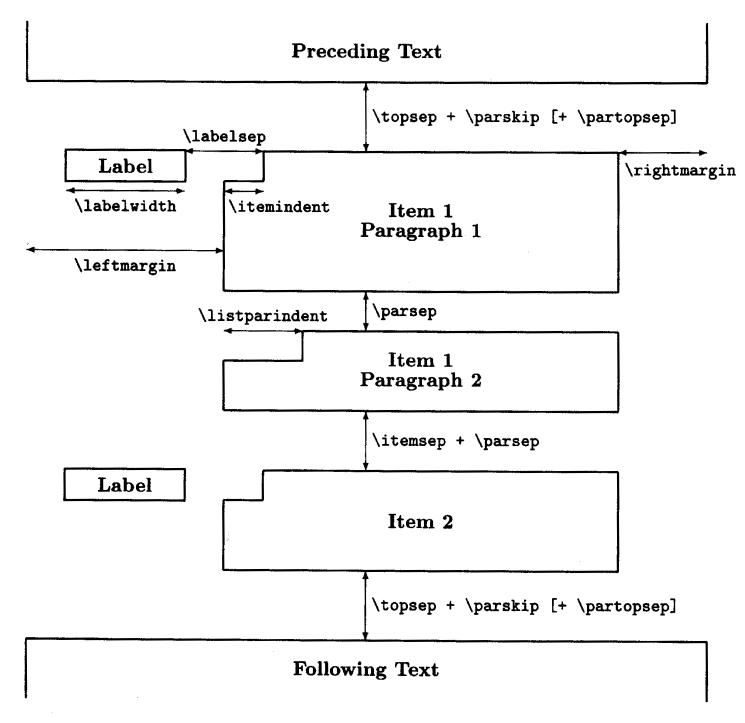
\includegraphics[scale=0.4]{list_layout}
\caption{引用自Leslie Lamport - A Document Preparation System\\
\centering Figure 6.3: The format of a list}
\end{figure}
%	\usecounter{counter} - 特定用于list环境的第二个参数, 可在列表中使用指定计数器
%	\topsep - 与partopsep、parskip组合, 称为外部文本与list的垂直距离(list上/下部分)
%	\partopsep - 与topsep、parskip组合, 成为外部文本与list的垂直距离, 默认为0pt
%	\labelsep - label与item首行的水平距离. label与item的距离为labelsep-itemindent
%	\itemindent - item首行缩进
%	\listparindent - item内, 除第一段的段落缩进
%	\parsep - item内, 段落之间的垂直间距
%	\itemsep - item之间, 指定的额外距离. 实际item之间的距离为itemsep+parsep
%	\leftmargin - item实际内容(label右侧文本内容)左侧距离外部文本内容左侧的水平距离
%	\rightmargin - item实际内容(label右侧文本内容)右侧距离外部文本内容右侧的水平距离
\end{document}
